%!TEX ROOT=formularioFisica.tex

\section{Appendice}
Questo formulario dá per scontate alcune nozioni matematiche. Di seguito sono riportate le più
basilari e importanti.

\subsection{Proporzionalità}
Per esprimere la proporzionalità si utilizza il simbolo $\propto$.\\
Si dicono \textbf{direttamente proporzionali} due variabili $x,y$ se
\begin{equation*}
  y = kx\,(y\propto x)
\end{equation*}
Ovvero se all'aumentare di $x$ aumenta anche $y$.\\ [\baselineskip]
Si dicono \textbf{inversamente proporzionali} due variabili $x,y$ se 
\begin{equation*}
  xy = k\,\left(y\propto\frac{1}{x}\right)
\end{equation*}

\subsection{Distanza}

La distanza tra due punti è un concetto fondamentale e si calcola 
\begin{equation*}
  d=\sqrt{(x2-x1)^{2}+(y2-y1)^{2}}
\end{equation*}
\begin{center}     
  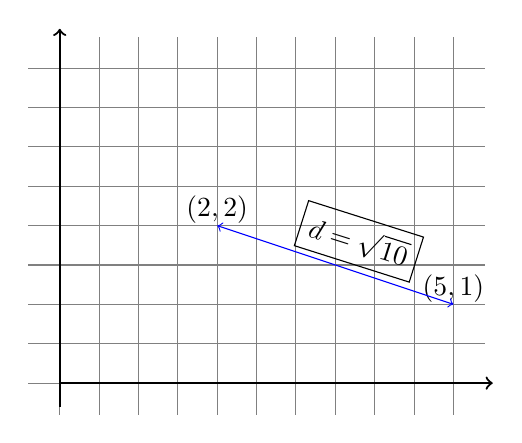
\begin{tikzpicture}
    \draw[step=0.5cm,gray](-0.9,-0.9) grid (4.9,3.9) ;
    \draw[thick,->,black] (-.5,-0.8) -- (-0.5,4) ;
    \draw[thick,->,black]  (-.5,-0.5)--(5,-0.5);
    \node at (1.5,1.7) {$(2,2)$};
    \node at (4.5,0.7){$(5,1)$};
    \draw[<->,blue](1.5,1.5)--(4.5,0.5);

    \node[draw,rotate=-17.6] at (3.3,1.3){$d=\sqrt{10}$};	
  \end{tikzpicture}            
\end{center}

\subsection{Notazione scientifica}
I valori ottenuti in fisica possono presentare a volte molti zeri, per ovviare alla difficoltà di 
lettura di questi numeri si utilizza la notazione scientifica che consiste nello scrivere qualunque
numero come 
\begin{equation*}
  \text{Numero}=x\cdot 10^{y}
\end{equation*}
con $x$ tra $0$ e $10$ e con ultima cifra diversa da $0$\\
Dunque $107,000=1,07\cdot10^{5}$ e $0.0000098=9,8\cdot10^{-8}$ 
Frequentemente $10^{y}$ viene ancora semplificato con alcuni prefissi:

\begin{center}
  \rowcolors{5}{green}{green}
  \begin{tabular}{c c c}
    & Prefisso & Nome prefisso\\ \hline
    $10^{18}$ & E &  esa\\ \hline
    $10^{15}$ & P & peta\\ \hline
    $10^{12}$ & T & tera\\ \hline
    $10^{9}$ & G & giga\\ \hline
    $10^{6}$ & M & mega\\ \hline
    $10^{3}$ & k & kilo\\ \hline
    $10^{2}$ & h & etto\\ \hline
    $10^{-1}$ & d & deci\\ \hline
    $10^{-2}$ & c & centi\\ \hline
    $10^{-3}$ & m & milli\\ \hline
    $10^{-6}$ & $\mu$ & micro\\ \hline 
    $10^{-9}$ & n & nano\\ \hline \hiderowcolors
    $10^{-12}$ & p & pico\\ \hline
    $10^{-15}$ & f & femto\\ \hline
    $10^{-18}$ & a & atto\\
  \end{tabular}
\end{center}

\subsection{Quadrato}
Il quadrato è una figura regolare con 4 lati.\\ Definendo $l=$lunghezza del lato si calcola
\begin{equation*}
  \text{Area}=l^{2}\quad\text{Diagonale}=l\sqrt{2}
\end{equation*}
\begin{center}     
  \begin{tikzpicture}
    \draw (0,0) -- (2,0) -- (2,2) -- (0,2) -- cycle;

    \node at (1,0.1) {$l$};
  \end{tikzpicture} 
\end{center}

\subsection{Triangolo}
Il triangolo è una figura con tre lati. Esistono svariati tipi di traingoli ma quelli piu comuni in 
fisica sono i trangoli rettangoli (ovvero quei triangoli che hanno un angolo di $90$ gradi).

\begin{center}     
  \begin{tikzpicture}
    \draw (0,0) -- (4,0);
    \node at (-0.15,-0.1) {C};
    \node at (2,1.1) {c};
    \draw (4,0) -- (0,2);
    \node at (4.2,-0.1) {A};
    \node at (-0.2,1) {a};
    \node at (3.5,0.1) {$\alpha$}; 
    \draw (0,2) -- (0,0);
    \node at (0,2.15) {B};
    \node at (0.175,1.7) {$\beta$};
    \node at (2,-0.2){b};
  \end{tikzpicture}
\end{center}
Si definisce $c$ (il lato più lungo) ipotenusa, $b$ (lato di media lunghezza) cateto maggiore e
$a$ (lato più corto)\\
Alla base di tutte le formule sul triangolo rettangolo sta il Teorema di Pitagora:
\begin{equation*}
  c^2=a^2+b^2
\end{equation*}
Oltre a questa formula sono fondamentali anche:
\begin{align*}
  b&=c\cos\alpha\quad\text{e}\quad a=c\sin\alpha\\
  a&=c\cos\beta\quad\text{e}\quad b=c\sin\beta
\end{align*}
Al seno e al coseno va aggiunta la tangente che si definisce:
\begin{equation*}
  \tan x = \frac{\sin x}{\cos x}
\end{equation*}
Attraverso la tangente:
\begin{equation*}
  a=b\tan\alpha \qquad
  b=a \tan\beta
\end{equation*}  
Un altra formula importante è
\vspace{-0.5cm}
\begin{center}
  \begin{equation*}
    \cos{x}^{2}+\sin{x}^{2}=1 
  \end{equation*}
\end{center}
che si usa per ottenere il il seno quando si ha il coseno e viceversa.
\subsection{Cerchio}

Il cerchio è una figura fondamentale, si dimostra che: 
\begin{align*}
  \text{Circonferenza}&=2\pi r\\
  \text{Area}&=\pi r^2
\end{align*}
\begin{center}     
  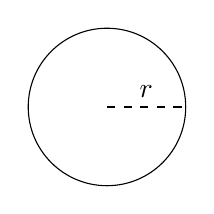
\begin{tikzpicture}
    \draw (0,0) circle (1cm);
    \draw [dashed](0,0)--(1,0);
    \node at (0.5,0.2) {$r$};
  \end{tikzpicture}
\end{center}
$\pi$ è un numero irrazionale definito appunto come rapporto la lunghezza della circonferenza e il 
diametro, il suo valore approssimato è $3,14159$. \\	
Facendo ruotare un cerchio di $180$ gradi si ottiene una sfera. Il volume di una sfera è pari a
\begin{equation*}
  V=\frac{4}{3}\pi r^3
\end{equation*}
La superficie invece
\begin{equation*}
  S = 4\pi r^2
\end{equation*}

\subsection{Equazioni}
Esistono svariati tipi di equazioni, tra le più comuni vi sono quelle di secondo grado. Per risolvere le equazioni   $ax^{2}+bx+c=0$  
si usa la seguente formula:

\begin{equation*}
  x_{1/2}={\frac{-b\pm\sqrt{b^{2}-4ac}}{2a}}
\end{equation*}
Per risolvere sistemi di equazioni come questo
\begin{equation*}
  \begin{cases}  ax+by= \textcolor{red}{c}, \\ dx+ey= \textcolor{red}{f},\\ 
  \end{cases}
\end{equation*}
si può usare il teorema di Cramer:

\begin{equation*}
  x=\dfrac{\begin{vmatrix}[1]
      \textcolor{red}{c} & b \\  
      \textcolor{red}{f} & e 
    \end{vmatrix}}{\begin{vmatrix}[1] 
  a & b \\ d & e \end{vmatrix}}= 
  \dfrac{\textcolor{red}{c}e-b\textcolor{red}{f}}{ae-bd}     \quad 
y=\dfrac{\begin{vmatrix}[1]  a &\textcolor{red}{c} \\ d &  \textcolor{red}{f} \end{vmatrix}}
{\begin{vmatrix}[1]  a & b \\ d & e \end{vmatrix}}= 
  \dfrac{a \textcolor{red}{f}- \textcolor{red}{c}d}{ae-bd}
\end{equation*}
Con questa logica si possono risolvere sistemi con anche più equazioni.

%!TEX ROOT=formularioFisica.tex

\section{Vettori}
Questa prima sezione � introduttiva ad uno dei concetti pi� comuni in fisica: il \emph{vettore}.\\
Un vettore pu� essere rappresentato in molti modi, tra cui:
\begin{equation*}
\vec{v} = 
\begin{bmatrix}[1]
a\\b\\\vdots
\end{bmatrix} = 
(a, b, \dots)
\end{equation*}
Un vettore � composto di un numero definito di \emph{componenti}, solitamente una per ciascuna
dimensione in cui si lavora. Quindi � decisamente pi� comune trovare vettori \emph{bidimensionali}
che non con un numero maggiore di componenti.\\
\begin{center}
	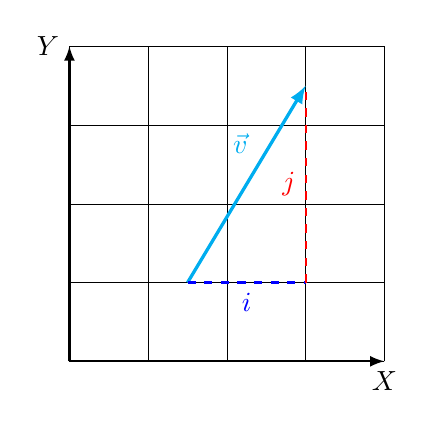
\begin{tikzpicture}
		\draw[step=1, very thin] (0,0) grid (4,4);
		\draw[-latex, thick] (0,0) -- (4,0)
			node[pos=1, below]{$X$};
		\draw[-latex, thick] (0,0) -- (0,4)
			node[pos=1, left]{$Y$};
		\draw[-latex, very thick, cyan] (1.5, 1) -- (3, 3.5)
			node[pos=0.6, above left]{$\vec{v}$};
		\draw[dashed, thick, blue] (1.5, 1) -- (3, 1)
			node[pos=0.5, below]{$i$};
		\draw[dashed, thick, red] (3, 1) -- (3, 3.5)
			node[pos=0.5, left]{$j$};
	\end{tikzpicture}
\end{center}
In questa immagine � possibile vedere un vettore $\mathcolor{cyan}{\vec{v}}(\mathcolor{blue}{i},
\mathcolor{red}{j})$ e le sue componenti.\\[\baselineskip]
D'ora in poi sar� dato per scontato che i vettori siano bi-dimensionali.

\subsection{Operazioni tra vettori}
Le operazioni come addizione e sottrazione funzionano molto semplicemente sommando algebricamente
le componenti tra di loro:
\begin{equation*}
\mathcolor{red}{\vec{v_1}\left(a_1, b_1\right)} \pm 
\mathcolor{blue}{\vec{v_2}\left(a_2, b_2\right)} = 
\mathcolor{purple}{\vec{v}}\left(\mathcolor{red}{a_1}\pm \mathcolor{blue}{a_2}, 
\mathcolor{red}{b_1}\pm \mathcolor{blue}{b_2}\right)
\end{equation*}

La moltiplicazione tra vettori pu� avere come risultato o un \emph{vettore} o uno \emph{scalare}.

\subsubsection{Prodotto scalare}
\begin{equation*}
\mathcolor{red}{\vec{v_1}} \cdot \mathcolor{blue}{\vec{v_2}} = 
\mathcolor{red}{a_1}\mathcolor{blue}{a_2} + \mathcolor{red}{b_1}\mathcolor{blue}{b_2}
\end{equation*}
Come si pu� notare il prodotto scalare tra due vettori torna uno scalare (ovvero un numero).
In fisica per� � molto pi� comune trovare questa definizione di prodotto scalare:
\begin{equation*}
\mathcolor{red}{\vec{v_1}} \cdot \mathcolor{blue}{\vec{v_2}} =
\norm{\mathcolor{red}{\vec{v_1}}}\cdot\norm{\mathcolor{blue}{\vec{v_2}}}\cos\theta
\end{equation*}
$\norm{\vec{v}}$ � il modulo del vettore $\vec{v}$, ovvero la sua lunghezza. $\theta$ � l'angolo
formato dai due vettori.

\subsubsection{Prodotto vettoriale}\label{subsec:vettori:prodottoVettoriale}
\begin{equation*}
\mathcolor{red}{\vec{v_1}} \times \mathcolor{blue}{\vec{v_2}} =
n\norm{\mathcolor{red}{\vec{v_1}}}\cdot\norm{\mathcolor{blue}{\vec{v_2}}}\sin\theta
\end{equation*}
$\norm{\vec{v}}$ � il modulo del vettore $\vec{v}$, ovvero la sua lunghezza. $\theta$ � l'angolo
formato dai due vettori. $n$ � la \emph{normale} del piano su cui stanno i vettori. Una \emph{normale}
� un vettore perpendicolare ad un oggetto dato.\\
Per scoprire la direzione del nuovo vettore si pu� usare la cos� detta 'regola della mano`. Essa dice:
\begin{enumerate}
	\item Usare il pollice della mano destra in direzione e verso del \textbf{primo} vettore
	\item Usare l'indice o le altre dite in direzione e verso del \textbf{secondo} vettore
	\item Il nuovo vettore avr� la direzione che attraversa il palmo perpendicolarmente e il verso 
	uscente dalla mano.
\end{enumerate}

\subsection{Percentuale}

La percentuale serve per esprimere delle informazioni numeriche, si esprime col simbolo \%.\\ 
N\% ha il significato di $\frac{N}{100}$. N\% di T è pari ad una parte di T (che va da 0 a T), 
per riassumere quindi 
\begin{equation*}
  T\cdot\frac{N}{100}=R
\end{equation*}
La variazione percentuale, serve a definire quando una quantità $x$ varia, è definita come:
\begin{equation*}
  \text{Variazione percentuale}=
  \frac{x_{\text{finale}}-x_{\text{iniziale}}}{x_{\text{iniziale}}}\cdot100
\end{equation*}
Quindi se la velocità di un corpo passsa da 15 m/s\\ a 20 m/s, vi è stato un aumento percentuale del 33,3\%.\\

\subsection{Esponenziali e logaritmi}
Esponenziali e logaritmi sono strettamente legati, come si può capire notando che:
\begin{equation*}
  \log_{a} b=x\qquad \qquad
  a^{x}=b
\end{equation*}
Molto spesso si utilizzerà questa caratteristica che deriva dalla definizione stessa di logaritmo:
\begin{equation*}
  a^{\log_{a}b}=b
\end{equation*}
Alcune proprietà delle espressioni esponenziali
\begin{align*}
  a^{b}\cdot a^{c}&=a^{bc}\\
  (a+b)^{c}&=a^{c}+b^{c}\\
  a^{-b}&=\frac{1}{a^{b}}
\end{align*}
Alcune propietà invece dei logaritmi sono
\begin{align*}
  \log_{a}(b*c)&=\log_{a}b+\log_{a}c\\
  \log_{a}\dfrac{b}{c}&=\log_{a}b-\log_{a}c\\
  \log_{a}(b^{c})&=c\log_{a}b
\end{align*}

\subsection{Derivate}
Le derivate sono una delle basi della fisica, infatti sono utilizzate per calcolare il valore di 
una varibile in un determinato tempo. Vengono definite in molti modi 
\begin{equation*}
  f'(t_0) \qquad
  \Dif f(t)_{t=t_0}\qquad
  \frac{\dif f}{\dif t}|_{t=t_0}\qquad
  \dot{f}
\end{equation*}
ma quello più comune in fisica è il terzo.\\
Prendiamo un esempio per capire cosa la derivata ricerchi.
\begin{center}
  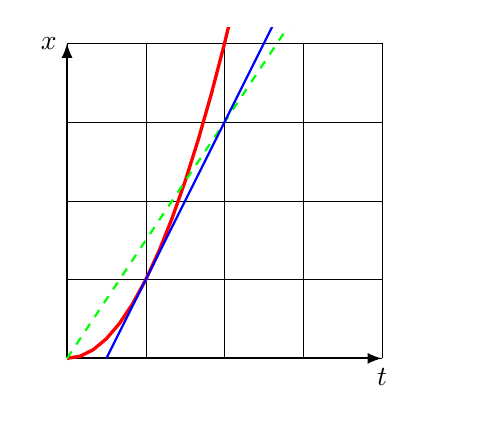
\begin{tikzpicture}[scale=1]
    \clip (-0.5,-0.5) rectangle (5,4.2);
    \draw[step=1, very thin] (0,0) grid (4,4);
    \draw[-latex, thick] (0,0) -- (4,0)
      node[pos=1, below]{$t$};
    \draw[-latex, thick] (0,0) -- (0,4)
      node[pos=1, left]{$x$};

    \draw[domain=0:4, very thick, red] plot(\x,{\x^2});
    \draw[domain=0:3, dashed, thick, green] plot(\x,{3/2*\x});
    \draw[domain=0.5:4, thick, blue] plot(\x, {2*\x-1});
  \end{tikzpicture}
\end{center}
La funzione (che descrive il moto di un corpo) è in rosso, in verde è rappresentata la velocità 
media tra $0$ e $2$ secondi e in blu invece è rappresentata la velocità istantanea a 1,5 secondi. 
La velocità istantanea in un determinato tempo è ottenuta con le derivate.\\
Sono diverse le formule per derivare una funzione ma quelle più usate sono:
\begin{align*}
  \frac{\dif k}{\dif x}&=0 &\quad \frac{\dif x^\alpha}{\dif x}&=\alpha x^{\alpha-1}\\
  \frac{\dif\sin x}{\dif x}&=\cos x & \frac{\dif\cos x}{\dif x}&=-\sin x\\
  \frac{\dif\log_ax}{\dif x}&=\frac{1}{x}\log_ae & \frac{\dif a^{x}}{\dif x}&=a^{x}\ln a
\end{align*}
A queste formule vanno aggiunti alcuni teoremi
\begin{align*}
  &\frac{\dif\left[k\cdot f(x) \right]}{\dif x}=k\frac{\dif f(x)}{\dif x}\qquad
  \frac{\dif[f(x)\pm g(x)]}{\dif x}=\frac{f(x)}{\dif x}\pm \frac{g(x)}{\dif x}\\
  &\frac{\dif [f(x)\cdot g(x)]}{\dif x}=\frac{\dif f(x)}{\dif x}g(x) + 
  f(x)\frac{\dif g(x)}{\dif x}\\
  &\frac{\dif \left[\frac{f(x)}{g(x)}\right]}{\dif x} =
  \frac{\frac{\dif f(x)}{\dif x}g(x)-f(x)\frac{\dif g(x)}{\dif x}}{[g(x)]^2}
\end{align*}
Un esempio: un corpo partendo da fermo cade dunque la sua posizione è descritta da 
$x=0.5\cdot9.81\cdot t^{2}$. La derivata della funzione è 
$\frac{\dif x}{\dif t}=0,5\cdot9,81\cdot2\cdot t$. 
Quindi la sua velocità dopo 3 secondi è pari a $29,4$m/s($0,5\cdot9,81\cdot3$).

\subsection{Integrale}
L'integrazione indefinita di $f(x)$ è  un operazione che determina tutte le funzioni $F(x)+k$ tali 
che $\frac{d(F(x)+k)}{dx}=f(x)$ ovvero $\int f(x)dx = F(x)+k$.\\
Queste sono le formule più ricorrenti dell'integrale definito: 
\begin{gather*}
  \int kf(x)\,\dif x=k \int f(x)\,\dif x+k\\ 
  \int\left[a(x)+b(x)\right] \dif x= \int a(x)\,\dif x + \int b(x)\,\dif x+k\\
  \int x^{\alpha}\,\dif x =\frac{x^{\alpha+1}}{\alpha+1}+k \\
  \int a^{x}\,\dif x=a^{x}\log_{a}e+k\\
  \int \sin(x)\,\dif x = -\cos(x)+k\\
  \int \cos(x)\,\dif x = \sin(x)+k\\
  \int \frac{1}{x}\,\dif x= \ln \abs{x}+k 
\end{gather*}
L'integrale definto invece è $\int_{a}^{b}=F(b)-F(a)$ dove a e b sono due punti finiti. 
L'area occupata da una funzione tra i punti a e b è 
\begin{equation*}
  A=(b-a)V_{\text{medio}}=\int_{a}^{b}f(x)\,\dif x
\end{equation*}
Si prenda ad esempio $y=\dfrac{1}{x}$ tra $a=1$ e $b=3$ 
\begin{center}
  \begin{tikzpicture}
    \clip (-0.5,-0.5) rectangle (5,4);
    \draw[-latex, thick] (0,0) -- (4.3,0)	
      node[pos=1, below]{$t$};	
    \draw[-latex, thick] (0,0) -- (0,3.3)	
      node[pos=1, left]{$x$};	
    \draw[domain=0.331:4, very thick, red] plot(\x,{\x^-1});	
    \node[blue] at (1,-.2) {a};
    \draw [red,dashed,thick] (1,0)--(1,1);
    \node[blue] at (3,-.2) {b};
    \draw[red,dashed,thick] (3,0)--(3,.4);
    \draw [white] (2,0.02)--(2,.48);
  \end{tikzpicture}
\end{center}
L'integrale indefinito è $\int \frac{1}{x}\,\dif x=\ln x+k$, l'area è dunque 
\begin{equation*}
  A=\int_{1}^{3} \frac{1}{x} dx =\ln(3)-\ln(1) \approx 1,01
\end{equation*}
